\chapter{Recognition of Bricks}
The recognition of the bricks is based on the the information of value, saturation and color given by the representation on the image in HSV color space.

The algorithm is illustrated with an example image taken in similar conditions as the workstation, \autoref{fig:RealLego4}.

\begin{figure}[H]
    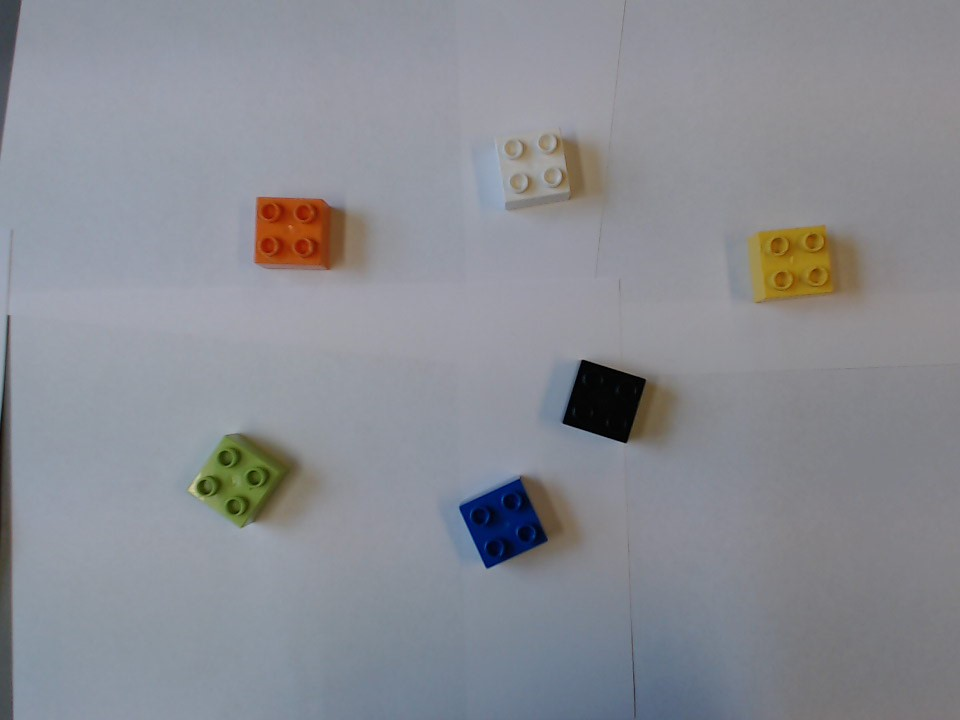
\includegraphics[width=0.4\textwidth]{figures/RealLego4.jpg}
    \caption{Original image that include the color bricks to recognize in random positions.}
    \label{fig:RealLego4}
\end{figure}

The first step is to convert the image to HSV color space and split the channels different channels.

To find the color blocks (orange, yellow, green and blue) the saturation channel is used combined with a threshold to find the pixels that have a high saturation value (bright colors). This step results in a binary mask, where the white pixels represent the object.

\begin{figure}[H]
    \captionbox  %<--use captionbox instead if no global caption is needed
    { 
        Saturation channel of the original image in HSV color space.              
        \label{fig:saturation}                                  
    }                                                                 
    {                                                                  
        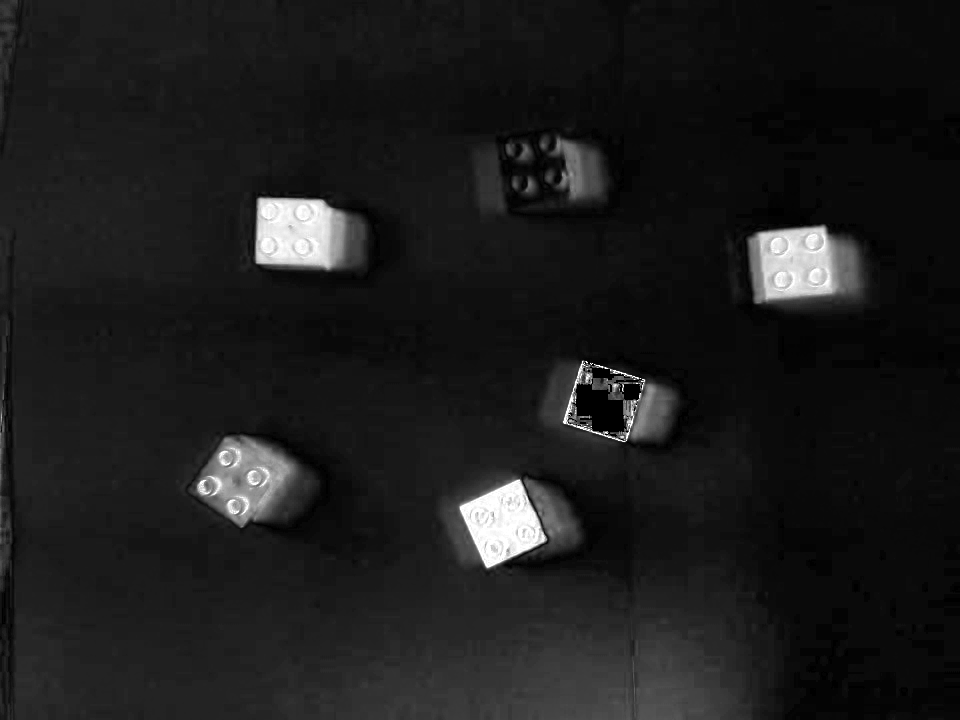
\includegraphics[width=.4\textwidth]{figures/saturation.png}         
    }                                                                    
    \hspace{5pt}                                                          
    \captionbox
    {      
        Mask for the color bricks (orange, green, blue and yellow). 
        \label{fig:colour_mask}                                     
    }
    {
        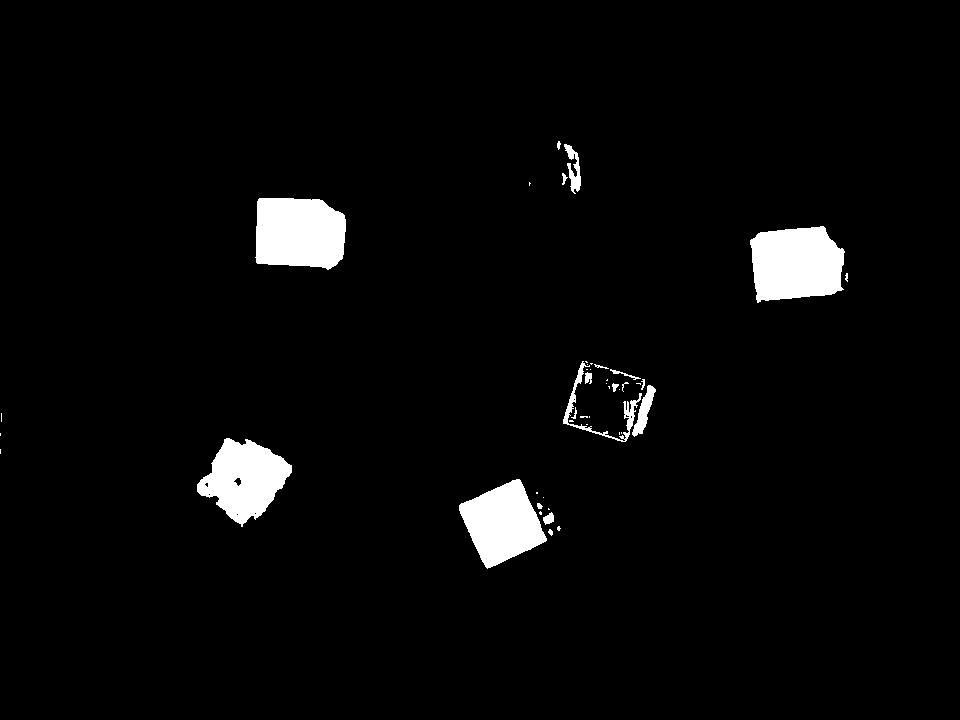
\includegraphics[width=.4\textwidth]{colour_mask.png}            
    }                                                                             
\end{figure}

To fin the black bricks, the value channel, \autoref{fig:value} can be used to find the pixels with very low value, that results in another mask, as seen in \autoref{fig:black_mask}.

\begin{figure}[H]
    \captionbox  %<--use captionbox instead if no global caption is needed
    {
        Value channel of the original image in HSV color space.                
        \label{fig:value}                                  
    }                                                                 
    {       
                                                                    
        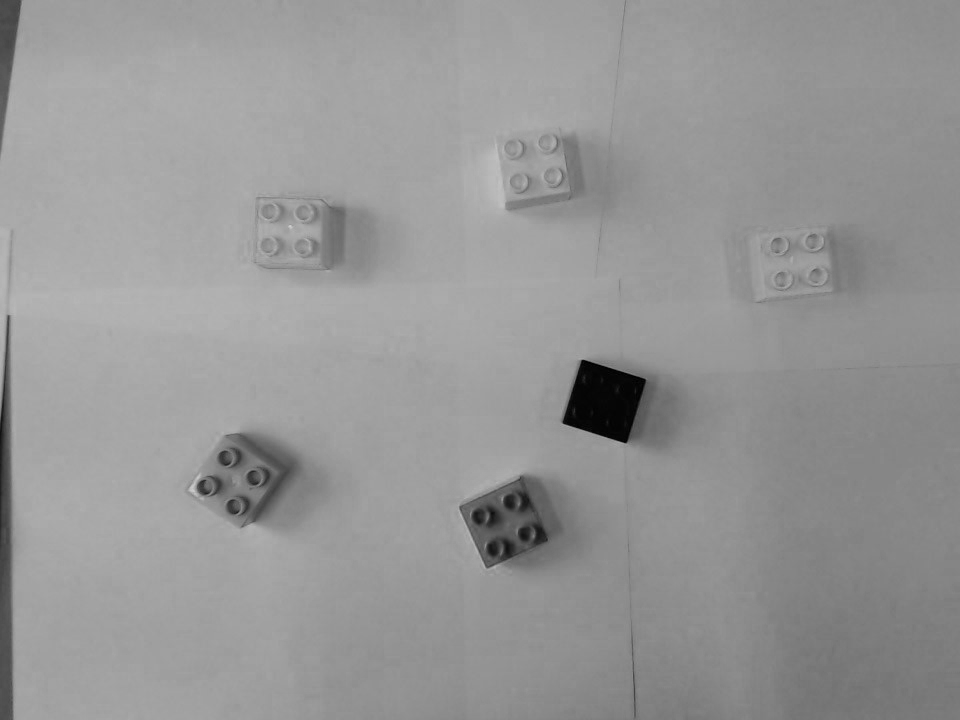
\includegraphics[width=.4\textwidth]{figures/value.png}         
    }                                                                    
    \hspace{5pt}                                                          
    \captionbox
    {  
        Mask for the black brick.
        \label{fig:black_mask}                                     
    }
    {
        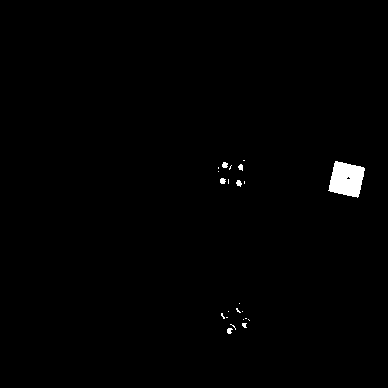
\includegraphics[width=.4\textwidth]{black_mask.png}            
    }                                                                             
\end{figure}

Combining the two masks, the final one can be found as seen in \autoref{fig:final_mask}. To enhance the mask, an opening operation to remove some of the noise, followed by a closing operation to fill possible holes in the objects. This operations give the result presented on \autoref{fig:final_mask2}.

\begin{figure}[H]
    \captionbox  %<--use captionbox instead if no global caption is needed
    {
        Combination of both masks before processing.             
        \label{fig:final_mask}                                  
    }                                                                 
    {                                                                  
        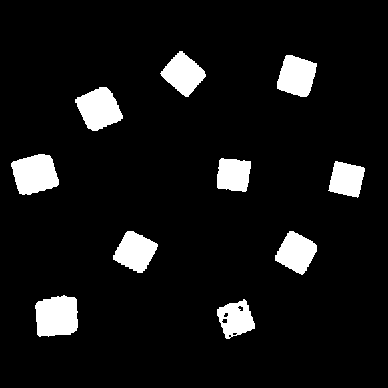
\includegraphics[width=.4\textwidth]{figures/final_mask.png}         
    }                                                                    
    \hspace{5pt}                                                          
    \captionbox
    {       
        Enhanced mask after removing noise and filling holes in the objects.
        \label{fig:final_mask2}                                     
    }
    {
        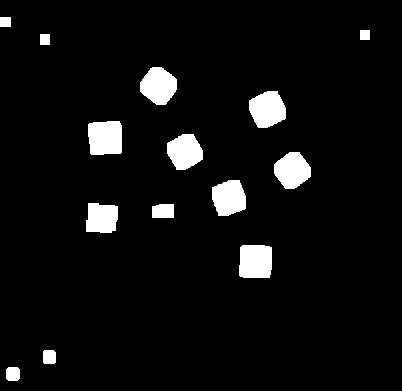
\includegraphics[width=.4\textwidth]{final_mask2.png}            
    }                                                                             
\end{figure}

Once the mask is enhanced, each of the objects can be labeled to be analyzed one by one. It is noticeable that only the objects that have an area larger than a threshold are considered for future processing.

The position of each brick can be found using the centroid of the pixels corresponding to each object, as seen in \autoref{fig:centroids}.

\begin{figure}[H]
    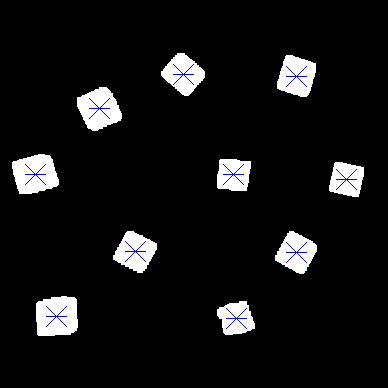
\includegraphics[width=0.4\textwidth]{figures/centroids.png}
    \caption{Centroids of the different objects in the mask (blue marks).}
    \label{fig:centroids}
\end{figure}

Once the position of the brick in the image is found, its color and orientation need to be stored as well to be used in further algorithms in the overall program.

The first one, the color, can be found looking at a small region around the center of each brick in the hue channel. The mean of the hue of these pixels is compared to four values corresponding to yellow, gree, blue and orange. The color of the object is selected as the one closer to the mean of the region.

To get the orientation is based on and edge detection followed by a Hough line transform. 

Since the image is already binary, \autoref{fig:object_mask}, the edges can be detected by calculating the difference between the image and a dilation of it. The result can be seen in \autoref{fig:edges}.


\begin{figure}[H]
    \captionbox  %<--use captionbox instead if no global caption is needed
    {
        Mask for one of the objects.              
        \label{fig:object_mask}                                  
    }                                                                 
    {                                                                  
        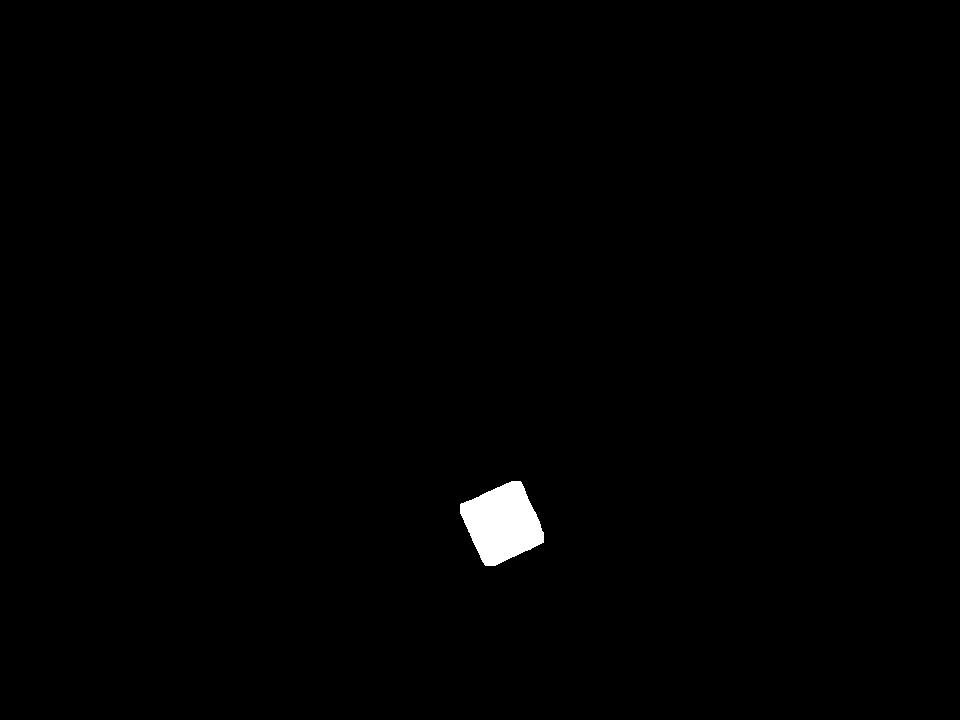
\includegraphics[width=.4\textwidth]{figures/object_mask.png}         
    }                                                                    
    \hspace{5pt}                                                          
    \captionbox
    {       
        Edges found in the object by the difference of the original mask and a dilated one.
        \label{fig:edges}                                     
    }
    {
        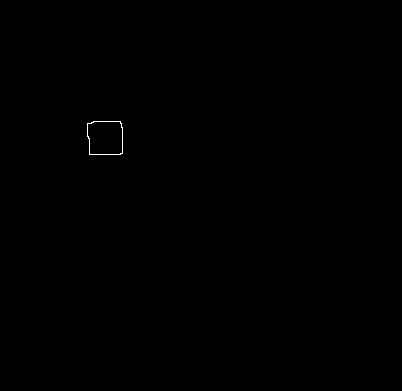
\includegraphics[width=.4\textwidth]{edges.png}            
    }                                                                              
\end{figure}

Once the edges are found, the Hough transform is used to find the lines. The orientation is defined by the angle of the largest line with respect to the horizontal, see \autoref{fig:object}.

\begin{figure}[H]
    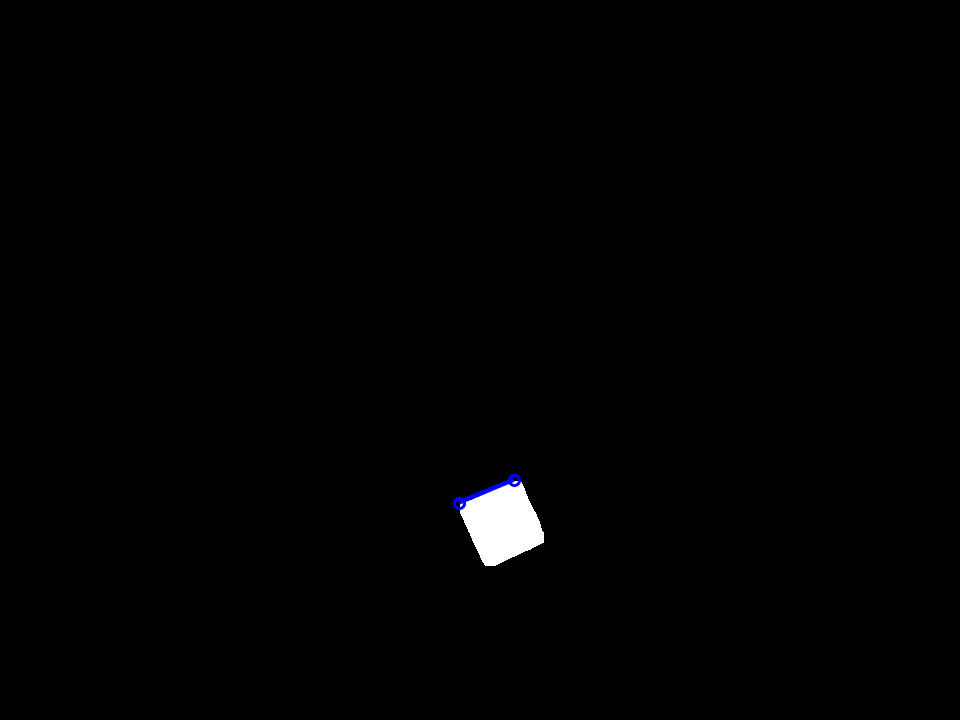
\includegraphics[width=0.4\textwidth]{figures/object.png}
    \caption{Largest line in the object marked in blue.}
    \label{fig:object}
\end{figure}

At this point, each brick is identified by its position in the image, its color and its orientation, so it is ready for being used in following algorithms.
